\newcommand{\height}{0}

\newcommand{\usualfigureheader}{
\begin{figure}
\begin{center}
\begin{pspicture}(0,0)(0,\height)
%\psline(-1,\height)(1,\height) \psline(0,\height)(0,-0.5)
}

\newcommand{\exclamatoryusualfigureheader}{
\begin{figure}[!!h]
\begin{center}
\begin{pspicture}(0, 0)(0, \height)
%\psline(-1,\height)(1,\height) \psline(0,\height)(0,0)
}

\input{presentation_text}
\input{deg_12_proof_macros}

\newcommand{\presentationfig}{
\renewcommand{\height}{17.5}
\usualfigureheader
%\psset{xunit=0.7cm, yunit=0.7cm}
\rput(-0.3,0){
%\rput(-6.9,-10.3){
\rput(-6.6,-10.3){
\includegraphics{presentation.eps}
\rput(1.2,27){
\rput[r](0,0){{\footnotesize $\mathit{0}$}}
\rput[r](0,-2.3){{\footnotesize $\mathit{5}$}}
\rput[r](0,-4.5){{\footnotesize $\mathit{10}$}}
\rput[r](0,-6.8){{\footnotesize $\mathit{15}$}}
}
}
\rput(-5.2, 7.5){\ptext}
}
\end{pspicture}
\renewcommand{\captionlabeldelim}{:}\caption{Illustration of a sample presentation file. Vertices $v$ with $(\gamma^-(v), \gamma^+(v)) = (5, \infty)$ are lightened for clarity.}\renewcommand{\captionlabeldelim}{}
\end{center}
\label{presentation}
\end{figure}
}

\newcommand{\fourintersectionfig}{
\renewcommand{\height}{3.6}
\usualfigureheader
%\psset{xunit=0.7cm, yunit=0.7cm}
\rput(-2,0.2){\includegraphics{four_intersection.eps}}
\end{pspicture}
\renewcommand{\captionlabeldelim}{:}\caption{How to make a map cubic.}\renewcommand{\captionlabeldelim}{}
\end{center}
\end{figure}
}

\newcommand{\mapandgraphfig}{
\renewcommand{\height}{3.6}
\usualfigureheader
%\psset{xunit=0.7cm, yunit=0.7cm}
\rput(0.5,0){\includegraphics{map_and_dual.eps}}
\end{pspicture}
\renewcommand{\captionlabeldelim}{:}\caption{Forming the dual graph of a map.}\renewcommand{\captionlabeldelim}{}
\end{center}
\end{figure}
}

\newcommand{\birkhoffdiamondfig}{
\renewcommand{\height}{2.7}
\usualfigureheader
%\psset{xunit=0.7cm, yunit=0.7cm}
\rput(0.55,-0.4){\includegraphics{birkhoffdiamond.eps}}
\end{pspicture}
\renewcommand{\captionlabeldelim}{:}\caption{The Birkhoff diamond $\gA$ (left) and its reducer $\gA'$ (right), shown with their dual maps.}\renewcommand{\captionlabeldelim}{}
\label{birkhoffdiamond}
\end{center}
\end{figure}
}

\newcommand{\degfivevertex}{
\psdot[dotsize=0.19]
}

\newcommand{\degsevenvertex}{
\pscircle[fillstyle=solid,fillcolor=white]{0.10}
}

\newcommand{\degeightvertex}{
\pspolygon[fillstyle=solid,fillcolor=white](-0.078,-0.078)(-0.078,0.078)(0.078,0.078)(0.078,-0.078)
}

\newcommand{\plus}{
\psline(-0.078, 0)(0.078, 0)
\psline(0, -0.078)(0, 0.078)
}

\newcommand{\degreetwelvefig}{
\renewcommand{\height}{13.4}
\usualfigureheader
\psset{linewidth=0.6pt}
\rput(2,-1){
\degtwelveproof
}
\end{pspicture}
\renewcommand{\captionlabeldelim}{:}\caption{The case analysis showing that a vertex of degree 7 cannot transfer more than $1/2$ units of charge to a vertex of degree $\geq 8$.}\renewcommand{\captionlabeldelim}{}
\label{degreetwelve}
\end{center}
\end{figure}
}

\newcommand{\vertexshapesfig}{
\renewcommand{\height}{1.7}
\usualfigureheader
\psset{linewidth=0.6pt}
\rput(-0.1,1.5){
\rput(-5,0){
\rput(0,0)   {\psline(0.19,-0.34)(0,0)(-0.19,-0.34)\psdot[dotsize=0.19]\rput(1.4,-0.08){degree 5}
\rput(0,-0.6){\psline(0.19,-0.34)(0,0)(-0.19,-0.34)\rput(1.4,-0.08){degree 6}
\rput(0,-0.6){\psline(0.19,-0.34)(0,0)(-0.19,-0.34)\pscircle[fillstyle=solid,fillcolor=white]{0.10}\rput(1.4,-0.08){degree 7}
}}}}
\rput(-1,0){
\rput(0,0)   {\psline(0.19,-0.34)(0,0)(-0.19,-0.34)\pspolygon[fillstyle=solid,fillcolor=white](-0.078,-0.078)(-0.078,0.078)(0.078,0.078)(0.078,-0.078)\rput(1.4,-0.08){degree 8}
\rput(0,-0.6){\psline(0.19,-0.34)(0,0)(-0.19,-0.34)\pspolygon[fillstyle=solid,fillcolor=white](-0.1,-0.07)(0,0.1)(0.1,-0.07)\rput(1.4,-0.08){degree 9}
\rput(0,-0.6){\psline(0.19,-0.34)(0,0)(-0.19,-0.34)\rput(0,-0.02){\pspolygon[fillstyle=solid,fillcolor=white](-0.061,-0.04)(-0.1,0.062)(0,0.14)(0.1,0.062)(0.061,-0.04)}\rput(1.5,-0.08){degree 10}
}}}}
\rput(2.8,0){
\rput(0,0)   {
\rput(0,-0.6){\psline(0.19,-0.34)(0,0)(-0.19,-0.34)\pspolygon[fillstyle=solid,fillcolor=white](-0.09,-0.09)(-0.09,0.09)(-0.03,0.09)(-0.03,-0.09)\rput(1.4,-0.08){degree 11}
                                                   \pspolygon[fillstyle=solid,fillcolor=white]( 0.09,-0.09)( 0.09,0.09)( 0.03,0.09)( 0.03,-0.09)
\rput(0,-0.6){
}}}}
}
\end{pspicture}
\renewcommand{\captionlabeldelim}{:}\caption{Shapes for showing the degree of a vertex.}\renewcommand{\captionlabeldelim}{}
\label{vertexshapes}
\end{center}
\end{figure}
}

\newcommand{\sqr}{0.866}
\newcommand{\sqrpp}{1.866}

\newcommand{\fivefivepairfig}{
\renewcommand{\height}{1.5}
\usualfigureheader
\psset{linewidth=0.8pt,xunit=0.69cm,yunit=0.69cm}
\rput(-6.2,1.3){
\pspolygon(-\sqr,0.5)(\sqr,-0.5)(\sqr,0.5)(-\sqr,-0.5)
\psdot[dotsize=0.19](-\sqr,-0.5)
\psdot[dotsize=0.19](-\sqr, 0.5)
\rput(1.732,0){
\psline(-\sqr,-0.5)(0,-1)(0,0)(-\sqr,0.5)
\psline(0,0)(-\sqr,-0.5)
\rput(-\sqr,-0.5){\pscircle[fillstyle=solid,fillcolor=white]{0.113}}
\psdot[dotsize=0.19](0,-1)
}
\rput(5.7,-.2){
\pspolygon(-1,0)(-0.5,-\sqr)(0.5,\sqr)(1.5,-\sqr)(2, 0)
\psdot[dotsize=0.19](0.5,\sqr)
\psline(-1,0)(-1.5,-\sqr)(-0.5,-\sqr)
\psline(2,0)(2.5,-\sqr)(1.5,-\sqr)
\psdot[dotsize=0.19](-1,0)
\psdot[dotsize=0.19](-1.5,-\sqr)
\psdot[dotsize=0.19](-0.5,-\sqr)
\psdot[dotsize=0.19](2,0)
\psdot[dotsize=0.19](2.5,-\sqr)
\psdot[dotsize=0.19](1.5,-\sqr)
\rput(5.7,0){
\psline(0,0)(-\sqr,0.5)(-\sqr,-0.5)(0,0)(1,0)(\sqrpp,0.5)(\sqrpp,-0.5)(1,0)
\psdot[dotsize=0.19](0,0)
\psdot[dotsize=0.19](1,0)
\psdot[dotsize=0.19](-\sqr,0.5)
\psdot[dotsize=0.19](-\sqr,-0.5)
\psdot[dotsize=0.19](\sqrpp,0.5)
\psdot[dotsize=0.19](\sqrpp,-0.5)
}
}
}
\end{pspicture}
\renewcommand{\captionlabeldelim}{:}\caption{Configurations with blocks of size 2 and 3. The first and third configurations have hanging 5-5 pairs.}\renewcommand{\captionlabeldelim}{}
\label{fivefivepair}
\end{center}
\end{figure}
}

\newcommand{\curvesfig}{
\renewcommand{\height}{1.8}
\usualfigureheader
\psset{xunit=0.7cm, yunit=0.7cm}
\rput(-4.3,0){\includegraphics{test.eps}}
\end{pspicture}
\renewcommand{\captionlabeldelim}{:}\caption{A potentially infinite sequence of $D$-reducible configurations, drawn in map form; terms of the sequence have been checked $D$-reducible up to ring-size 18 (the first configuration has ring-size 9).}\renewcommand{\captionlabeldelim}{}
\end{center}
\end{figure}
}

\newcommand{\mayerfig}{
\renewcommand{\height}{5.1}
\usualfigureheader
%\psset{xunit=0.7cm, yunit=0.7cm}
\rput(-3.4,0){\includegraphics{mayer.eps}
  %\rput(-.15,4.52){
  %\rput(-0.6,0){{\Large{\textbf{1}}}}
  %\rput(0.8,0.40){$\frac{1}{10}$}
  %\rput(0.8,-0.42){$\frac{1}{10}$}
  %\rput(0.19,-1.27){$\frac{1}{10}$}
  %\rput(-0.75,-1.62){$\frac{1}{10}$}
  %\rput(-1.74,-1.23){$\frac{1}{10}$}
  %\rput(-2.23,-0.53){$\frac{1}{10}$}
  %\rput(-2.23, 0.49){$\frac{1}{10}$}
  %\rput(-1.75, 1.26){$\frac{1}{10}$}
  %\rput(0.22, 1.28){$\frac{1}{10}$}
  %\rput(-0.75, 1.61){$\frac{1}{10}$}
  %}
  \rput(-.15,3.78){
    %\psline(-1,0)(1,0)
  \rput(-0.7,0){{\large{\textbf{1}}}}
  \rput(0.43,0.32){$\frac{1}{10}$}
  \rput(0.43,-0.3){$\frac{1}{10}$}
  \rput(-0.05,-1.02){$\frac{1}{10}$}
  \rput(-0.75,-1.28){$\frac{1}{10}$}
  \rput(-1.58,-0.95){$\frac{1}{10}$}
  \rput(-1.95,-0.42){$\frac{1}{10}$}
  \rput(-1.95, 0.42){$\frac{1}{10}$}
  \rput(-1.58, 1.02){$\frac{1}{10}$}
  \rput(-0.75, 1.32){$\frac{1}{10}$}
  \rput(-0.05, 1.1){$\frac{1}{10}$}
  }
}
\end{pspicture}
\renewcommand{\captionlabeldelim}{:}\caption{A sketch of Mayer's discharging procedure, using map form. Top: a pentagon divides its charge of 1 into 10 packets and sends two packets to each neighbor. A packet settles if the neighbor is a major vertex, otherwise travels clockwise or counterclockwise around the neighbor until it reaches a major vertex or until a reducible configuration appears. Bottom: sample packet trajectories. In the third drawing, the charge stops because of the appearance of a reducible configuration (the fifth configuration of Fig$.$ \ref{minorconfs}). In the fourth drawing, the charge would stop before the heptagon if Bernhart's diamond (Fig$.$ \ref{bernhart}) were an allowed configuration. If no major vertex appears one of the configurations of Fig$.$ \ref{minorconfs} necessarily appears.}\renewcommand{\captionlabeldelim}{}
\label{mayerrules}
\end{center}
\end{figure}
}

\newcommand{\minorconfsfig}{
\renewcommand{\height}{2.4}
\usualfigureheader
\rput(-7.35,0.5){\includegraphics{minor.eps}}
\end{pspicture}
\renewcommand{\captionlabeldelim}{:}\caption{The $D$-reducible configurations used for Mayer's discharging procedure.}\renewcommand{\captionlabeldelim}{}
\label{minorconfs}
\end{center}
\end{figure}
}

\newcommand{\proofconfsfig}{
\renewcommand{\height}{3.4}
\usualfigureheader
\rput(-6.8,1.25){\includegraphics{proofconfs.eps}}
\end{pspicture}
\renewcommand{\captionlabeldelim}{:}\caption{The $D$-reducible configurations used for the proof of Lemma \ref{lastly}.}\renewcommand{\captionlabeldelim}{}
\label{proofconfs}
\end{center}
\end{figure}
}

\newcommand{\bernhartfig}{
\renewcommand{\height}{1.0}
\usualfigureheader
\psset{xunit=0.9cm,yunit=0.9cm}
\rput(0,0.4){
\pspolygon[linewidth=0.7pt](0,0.5)(0.866,0)(0,-0.5)(-0.866,0)
\psline(0,0.5)(0,-0.5)
\psdot[dotsize=0.2](0.866,0)
\psdot[dotsize=0.2](-0.866,0)
}
\end{pspicture}
\renewcommand{\captionlabeldelim}{:}\caption{The Bernhart diamond, a $C$-reducible configuration.}\renewcommand{\captionlabeldelim}{}
\label{bernhart}
\end{center}
\end{figure}
}

\newcommand{\rsstrulesfig}{
\renewcommand{\height}{13.6}
\usualfigureheader
\psset{xunit=0.7cm, yunit=0.7cm}
\rput(-9.7,-16.7){
\rput(0.5,-1.5){\includegraphics{rules_rsst_0.eps}}}
\end{pspicture}
\renewcommand{\captionlabeldelim}{:}\caption{The discharging rules of Roberston et al.}\renewcommand{\captionlabeldelim}{}
\label{rsstrules}
\end{center}
\end{figure}
}

\newcommand{\mainrulesfig}{
\renewcommand{\height}{16.1}
\usualfigureheader
\psset{xunit=0.7cm, yunit=0.7cm}
\rput(-10.4,-13){
\rput(0.7,-1.5){\includegraphics{rulesMain_0.eps}}}
\end{pspicture}
\renewcommand{\captionlabeldelim}{:}\caption{Our set of discharging rules, $\mcal{L}_{42}$.}\renewcommand{\captionlabeldelim}{}
\label{mainrules}
\end{center}
\end{figure}
}

\newcommand{\wellpositionedfig}{
\renewcommand{\height}{3}
\usualfigureheader
\psset{xunit=0.7cm, yunit=0.7cm}
\rput(-3.8, 1){
\rput(0.5,-1.5){\includegraphics{wellpositioned.eps}}}
\end{pspicture}
\renewcommand{\captionlabeldelim}{:}\caption{The configuration in bold appears in every cartwheel fitting the drawn part but is never well-positioned. Vertices with $\gamma_P^+(v) = \infty$ are lightened for clarity.}\renewcommand{\captionlabeldelim}{}
\label{wellpositioned}
\end{center}
\end{figure}
}

\newcommand{\spanningtreefig}{
\renewcommand{\height}{1.5}
\usualfigureheader
\psset{xunit=0.7cm, yunit=0.7cm}
\rput(0,1){\psline[linewidth=1.3pt,arrowsize=0.22]{->}(-0.8,0)(0.8,0)}
\rput(-7, -0.1){
\rput(0.3,-1.5){\includegraphics{spanning_tree.eps}}}
\end{pspicture}
\renewcommand{\captionlabeldelim}{:}\caption{Preparing a spanning tree of faces.}\renewcommand{\captionlabeldelim}{}
\label{spanningtree}
\end{center}
\end{figure}
}

\newcommand{\bigradiusesfig}{
\renewcommand{\height}{1.5}
\usualfigureheader
\psset{xunit=0.7cm, yunit=0.7cm}
\rput(-9.4, -0.1){
\rput(0.3,-1.5){\includegraphics{bigradiuses.eps}}}
\end{pspicture}
\renewcommand{\captionlabeldelim}{:}\caption{Some $D$-reducible configurations of radius greater than two that fit in a second neighborhood.}\renewcommand{\captionlabeldelim}{}
\label{bigradiuses}
\end{center}
\end{figure}
}

\newcommand{\unencodablefig}{
\renewcommand{\height}{1.3}
\usualfigureheader
\psset{xunit=0.7cm, yunit=0.7cm}
\rput(-2.3, 0.8){
\rput(0.3,-1.5){\includegraphics{unencodable.eps}}}
\end{pspicture}
\renewcommand{\captionlabeldelim}{:}\caption{A rule that cannot be encoded as a part.}\renewcommand{\captionlabeldelim}{}
\label{unencodable}
\end{center}
\end{figure}
}
